\documentclass{article}
\usepackage{amsmath}
\usepackage{amssymb}
\usepackage{enumerate}
\usepackage{pgfplots}

\makeatletter
\renewcommand{\abstractname}{Instructions}
\makeatother

\pgfplotsset{holdot/.style={color=blue,fill=white,only marks,mark=*}}

\title{MAT -- 112: Calculus I and Modeling\\
\large{EFY 4}}
\author{Thomas R. Cameron}
\date{February 8, 2018}

\begin{document}
\maketitle

\begin{abstract}
Please complete each of the following problems. You should work independently, but you may receive help from your peers or myself. Be sure that you turn in your work before the end of class today. 
\end{abstract}

\paragraph*{Problem 1.}	For each graph below, provide a plot of $f^{'}$. 
\begin{enumerate}[(\alph{enumi})]
\item ~\\
\begin{figure}[h]
\centering
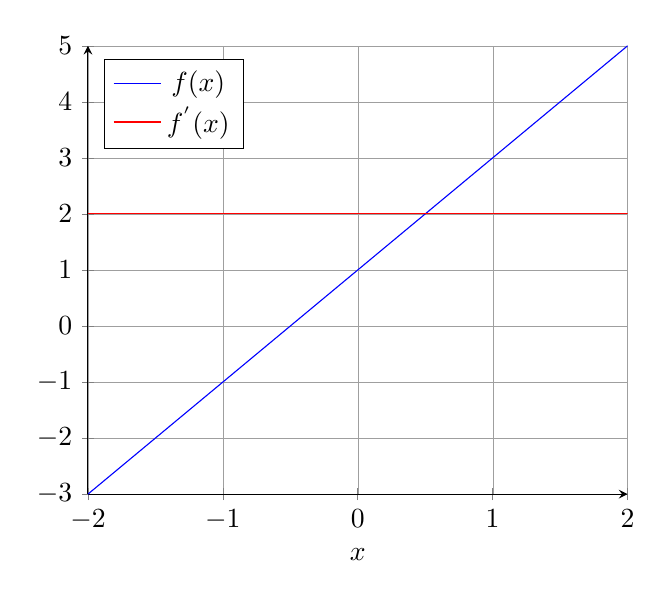
\begin{tikzpicture}
\begin{axis}[
	axis lines = left,
	legend pos = north west,
	xlabel = $x$,
	xtick={-2,...,2},
	ytick={-3,...,5},
	grid = both,
	grid style = {line width=0.1pt, draw=gray!75},
]
\addplot [
	domain = -2:2,
	samples = 200,
	color = blue,
]
{2*x+1};
\addlegendentry{$f(x)$}
\addplot [
	domain = -2:2,
	samples = 200,
	color = red,
]
{2};
\addlegendentry{$f^{'}(x)$}
\end{axis}
\end{tikzpicture}
\end{figure}~\\
\newpage
\item	~\\
\begin{figure}[h]
\centering
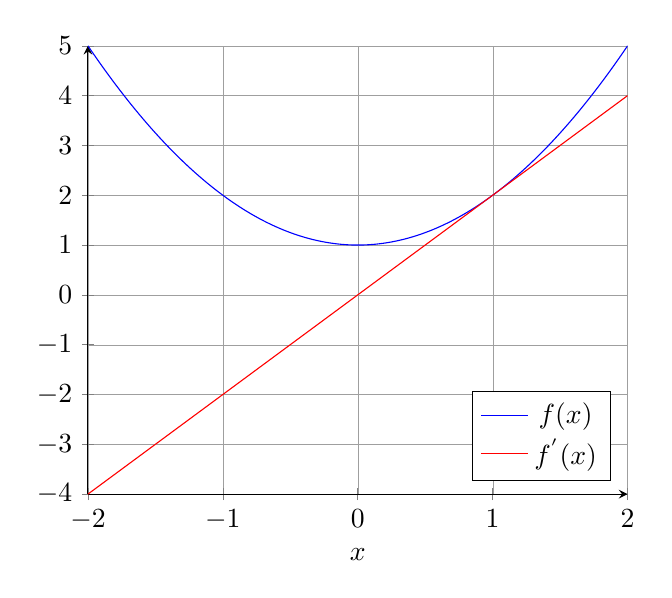
\begin{tikzpicture}
\begin{axis}[
	axis lines = left,
	legend pos = south east,
	xlabel = $x$,
	ymin = -4, ymax = 5,
	xtick={-2,...,2},
	ytick={-4,...,5},
	grid = both,
	grid style = {line width=0.1pt, draw=gray!75},
]
\addplot [
	domain = -2:2,
	samples = 200,
	color = blue,
]
{x^2+1};
\addlegendentry{$f(x)$}
\addplot [
	domain = -2:2,
	samples = 200,
	color = red,
]
{2*x};
\addlegendentry{$f^{'}(x)$}
\end{axis}
\end{tikzpicture}
\end{figure}~\\

\item ~\\
\begin{figure}[h]
\centering
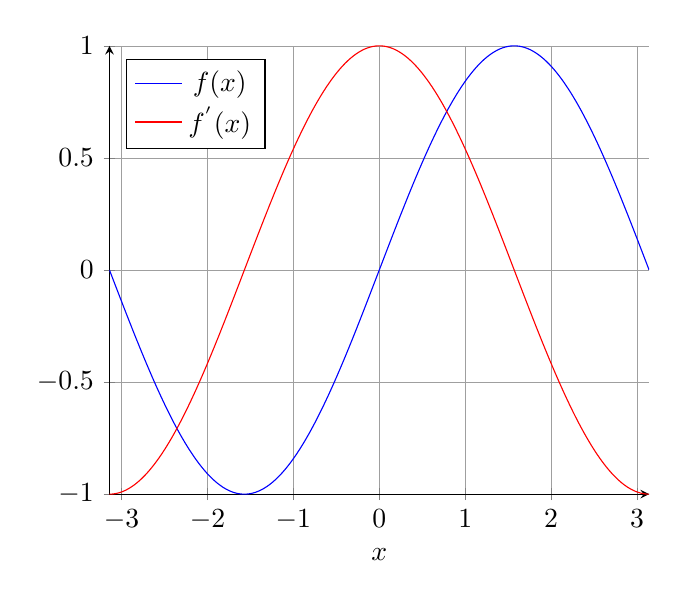
\begin{tikzpicture}
\begin{axis}[
	axis lines = left,
	legend pos = north west,
	xlabel = $x$,
	xtick={-4,...,4},
	ytick={-1,-0.5,0,0.5,1},
	grid = both,
	grid style = {line width=0.1pt, draw=gray!75},
]
\addplot [
	domain = -pi:pi,
	samples = 200,
	color = blue,
]
{sin(deg(x))};
\addlegendentry{$f(x)$}
\addplot [
	domain = -pi:pi,
	samples = 200,
	color = red,
]
{cos(deg(x))};
\addlegendentry{$f^{'}(x)$}
\end{axis}
\end{tikzpicture}
\end{figure}~\\
What function does the plot of $f^{'}$ resemble? \emph{The plot resembles $\cos(x)$.}
\end{enumerate}
\newpage
\paragraph*{Problem 2.} For each graph below, provide a plot of $f^{'}$. In addition, identify points where the derivative does not exist and provide explanation.
\begin{enumerate}[(\alph{enumi})]
\item	~\\
\begin{figure}[h]
\centering
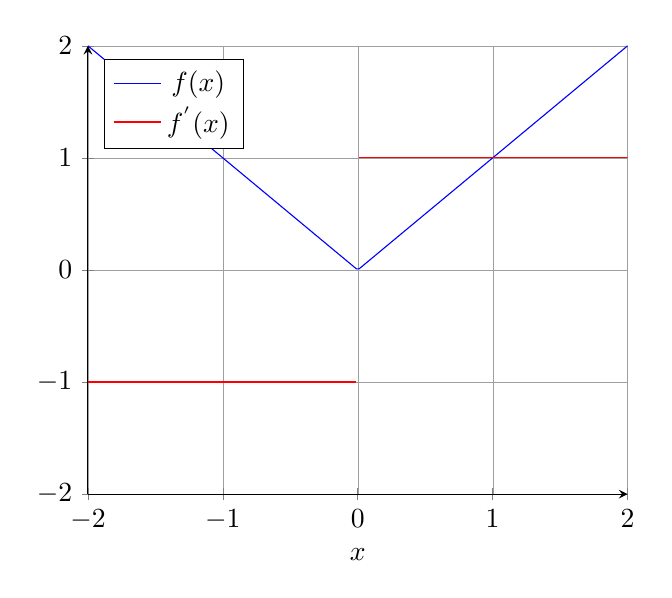
\begin{tikzpicture}[
	declare function = {
		g(\x) = (\x<0) * (-1) + 
			(\x>0) * (1);
	}
]
\begin{axis}[
	axis lines = left,
	legend pos = north west,
	xlabel = $x$,
	ymin = -2, ymax = 2,
	xtick={-2,...,2},
	ytick={-2,...,2},
	grid = both,
	grid style = {line width=0.1pt, draw=gray!75},
]
\addplot [
	domain = -2:2,
	samples = 200,
	color = blue,
]
{abs(x)};
\addlegendentry{$f(x)$}
\addplot [
	domain = -2:-0.01,
	samples = 200,
	color = red,
]
{g(x)};
\addplot [
	domain = 0.01:2,
	samples = 200,
	color = red,
]
{g(x)};
\addlegendentry{$f^{'}(x)$}
\end{axis}
\end{tikzpicture}
\end{figure}~\\
\emph{The derivative is not defined at $x=0$}.
\item	~\\
\begin{figure}[h]
\centering
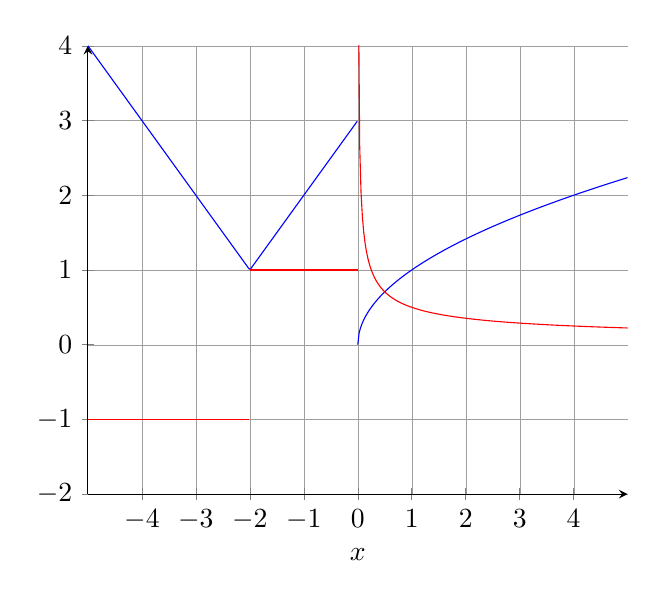
\begin{tikzpicture}[
	declare function={
		f(\x)= (\x<0) * (abs(\x+2)+1) +
			 (\x>=0) * (sqrt(\x));
		g(\x) = (\x<-2) * (-1) +
		and	(\x>-2, \x<0) * (1) +
			(\x>0) * (0.5/sqrt(\x));
	}
]
\begin{axis}[
	axis lines = left,
	legend pos = north east,
	xlabel = $x$,
	ymin = -2, ymax = 4,
	xtick = {-4,...,4},
	ytick = {-2,...,4},
	grid = both,
	grid style = {line width=0.1pt, draw=gray!75},
]
\addplot [
	domain = -5:-0.01,
	samples = 200,
	color = blue,
]
{f(x)};
\addplot [
	domain = 0:5,
	samples = 200,
	color = blue,
]
{f(x)};
\addplot [
	domain = -5:-2.01,
	samples = 200,
	color = red,
]
{g(x)};
\addplot [
	domain = -1.99:-0.01,
	samples = 200,
	color = red,
]
{g(x)};
\addplot [
	domain = 0.01:5,
	samples = 200,
	color = red,
]
{g(x)};
\end{axis}
\end{tikzpicture}
\end{figure}~\\
\emph{The derivative is note defined at $x=-2$ and $x=0$}.
\item ~\\
\begin{figure}[h]
\centering
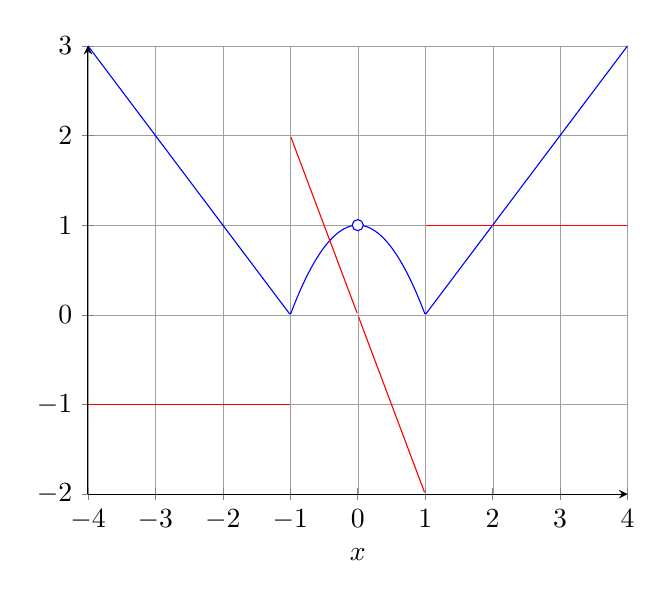
\begin{tikzpicture}[
	declare function={
		f(\x)= (\x<-1) * (-\x-1) +
		and	(\x>=-1, \x<1) * (1-\x^2) +
			(x>1) * (\x-1);
		g(\x) = (\x<-1) * (-1) +
		and	(\x>-1, \x<1) * (-2*\x) +
			(\x>1) * (1);	
	}
]
\begin{axis}[
	axis lines = left,
	legend pos = north east,
	xlabel = $x$,
	ymin = -2, ymax = 3,
	xtick = {-4,...,4},
	ytick = {-2,...,3},
	grid = both,
	grid style = {line width=0.1pt, draw=gray!75},
]
\addplot [
	domain = -4:-0.01,
	samples = 200,
	color = blue,
]
{f(x)};
\addplot [holdot] coordinates{(0,1)};
\addplot [
	domain = 0.01:4,
	samples = 200,
	color = blue,
]
{f(x)};
\addplot [
	domain = -4:-1.01,
	samples = 200,
	color = red,
]
{g(x)};
\addplot [
	domain = -0.99:-0.01,
	samples = 200,
	color = red,
]
{g(x)};
\addplot [
	domain = 0.01:0.99,
	samples = 200,
	color = red,
]
{g(x)};
\addplot [
	domain = 1.01:4,
	samples = 200,
	color = red,
]
{g(x)};
\end{axis}
\end{tikzpicture}
\end{figure}~\\
\emph{The derivative is not defined at $x=-1$, $x=0$, and $x=1$}.
\end{enumerate}

\end{document}